%%%%%%%%%%%%%%%%%%%%%%%%%%%%%%%%%%%%%%%%%%%%%%%%%%%%%%%%%%%%%%%%%%%%%%
% LaTeX Example: Project Report
%
% Source: http://www.howtotex.com
%
% Feel free to distribute this example, but please keep the referral
% to howtotex.com
% Date: March 2011 
% 
%%%%%%%%%%%%%%%%%%%%%%%%%%%%%%%%%%%%%%%%%%%%%%%%%%%%%%%%%%%%%%%%%%%%%%
% How to use writeLaTeX: 
%
% You edit the source code here on the left, and the preview on the
% right shows you the result within a few seconds.
%
% Bookmark this page and share the URL with your co-authors. They can
% edit at the same time!
%
% You can upload figures, bibliographies, custom classes and
% styles using the files menu.
%
% If you're new to LaTeX, the wikibook is a great place to start:
% http://en.wikibooks.org/wiki/LaTeX
%
%%%%%%%%%%%%%%%%%%%%%%%%%%%%%%%%%%%%%%%%%%%%%%%%%%%%%%%%%%%%%%%%%%%%%%
% Edit the title below to update the display in My Documents
%\title{343 Assignment 2}
%
%%% Preamble
\documentclass[paper=a4, fontsize=11pt]{scrartcl}
\usepackage[T1]{fontenc}
\usepackage{fourier}

\usepackage[english]{babel}															% English language/hyphenation
\usepackage[protrusion=true,expansion=true]{microtype}	
\usepackage{amsmath,amsfonts,amsthm} % Math packages
\usepackage{mathtools}
\usepackage[pdftex]{graphicx}	
\usepackage{url}
\usepackage{ulem}

\DeclarePairedDelimiter\floor{\lfloor}{\rfloor}
\DeclarePairedDelimiter\ceil{\lceil}{\rceil}


\newtheorem{theorem}{Theorem}

%%% Custom sectioning
\usepackage{sectsty}
\allsectionsfont{\centering \normalfont\scshape}


%%% Custom headers/footers (fancyhdr package)
\usepackage{fancyhdr}
\pagestyle{fancyplain}
\fancyhead{}											% No page header
\fancyfoot[L]{}											% Empty 
\fancyfoot[C]{}											% Empty
\fancyfoot[R]{\thepage}									% Pagenumbering
\renewcommand{\headrulewidth}{0pt}			% Remove header underlines
\renewcommand{\footrulewidth}{0pt}				% Remove footer underlines
\setlength{\headheight}{13.6pt}


%%% Equation and float numbering
\numberwithin{equation}{section}		% Equationnumbering: section.eq#
\numberwithin{figure}{section}			% Figurenumbering: section.fig#
\numberwithin{table}{section}				% Tablenumbering: section.tab#


%%% Maketitle metadata
\newcommand{\horrule}[1]{\rule{\linewidth}{#1}} 	% Horizontal rule

\title{
		%\vspace{-1in} 	
		\usefont{OT1}{bch}{b}{n}
		\normalfont \normalsize \textsc{Institute of Technology} \\ [25pt]
		\horrule{0.5pt} \\[0.4cm]
		\huge TCSS 343 - Assignment 2\\
		\horrule{2pt} \\[0.5cm]
}
\author{
		\normalfont 								\normalsize
        Version 1.0\\[-3pt]
}


%%% Begin document
\begin{document}
\maketitle

\section{Guidelines}
Homework should be electronically submitted to the instructor by midnight on the due date.  A submission link is provided on the course Canvas Page.  The submitted document should be typeset using any common software and submitted as a PDF.  We strongly recommend using \LaTeX\;  to prepare your solution.  You could use any \LaTeX\; tools such as Overleaf, ShareLatex, TexShop etc. Scans of handwritten/hand drawn solutions are acceptable, but you will be docked 1 point per problem if the handwritting is unclear.

Each problem is worth a total of 20 points except the challenge problem which is worth 10 points.  Solutions receiving full points must be correct (no errors or omissions), clear (stated in a precise and concise way), and have a well organized presentation.  Show your work as partial points will be awarded to rough solutions or solutions that make partial progress toward a correct solution.

\textbf{Remember to cite} all sources you use other than the text, course material or your notes.

\newpage
\section{Problems}

\subsection{Understand}

For this problem consider the problem of finding the maximum element in a list of integers.

\vspace{12pt}

\noindent\texttt{Maximum Integer in a List (MAX)}

\texttt{Input: A list of integers $A[a...b]$.}

\texttt{Output: $A[i]$ for some $a\leq i\leq b$ such that $A[i] \geq A[j]$ for all $a \leq j \leq b$.}
\vspace{12pt}

\noindent Let $M(A[a...b])$ represent the output of the \texttt{MAX} problem on input $A[a...b]$.  Let Max($a$,$b$) be a simple function that returns the maximum of two elements.  Let $m = \left\lfloor\frac{a+b}{2}\right\rfloor$ be the midpoint between $a$ and $b$.


\begin{enumerate}
\item [(3 points) 1.] Below is a self-reduction for the \texttt{MAX} problem.  State a recursive algorithm using pseudocode for finding the maximum element based on this self-reduction.

\[
M(A[a...b]) = \left\{
\begin{tabular}{cc}
A[a] & \text{if} $a = b$ \\
$\text{Max}(A[a],M(A[a+1...b]))$ & \text{if} $a<b$ \\
\end{tabular}\right.
\]

\textbf{Recursive algorithm:}

findMax($A[a...b]$) 
	
\hspace{5ex} If $a=b$, return $A[a]$.

\hspace{5ex} Let $c=$ findMax($A[a+1\dots b]$).

\hspace{5ex} Return Max($A[a]$, $c$).

End findMax



\item [(2 points) 2.] Using the same reduction as part 1 now state a recurrence $T(n)$ that expresses the worst case run time of the recursive algorithm.  Find a similar recurrence in your notes and state the tight bound on $T(n)$ (you do not need to prove this bound).

\[
T(n) = \left\{
\begin{tabular}{cc}
	c & if $n \leq 1$ \\
	T(n-1) + d & if $n > 1$
\end{tabular}\right.
\]

\textbf{Tight bound:}

$an$ when $a=min\{c, d\} \leq T(n) \leq b(n)$ when $b=max\{c,d\}$.




\item [(3 points) 3.] Below is a self-reduction for the \texttt{MAX} problem.  State a recursive algorithm using pseudocode for finding the maximum element based on this self-reduction.

\[
M(A[a...b]) = \left\{
\begin{tabular}{cc}
$-\infty$ & \text{if} $a > b$ \\
$A[a]$ & \text{if} $a = b$ \\
$\text{Max}(A[m], \text{Max}(M(A[a...m-1]),M(A[m+1...b]))$ & \text{if} $a<b$ \\
\end{tabular}\right.
\]

\textbf{Recursive algorithm:}

findMax(A[a\dots b])

\hspace{5ex} If $a>b$ return $-\infty$.

\hspace{5ex} If $a=b$ return $A[a]$.

\hspace{5ex} Let $m=\floor{\frac{a+b}{2}}$.

\hspace{5ex} Let $c=$findMax$(A[m+1...b])$.

\hspace{5ex} Let $d=$findMax$(A[a...m-1])$.

\hspace{5ex} return Max$(A[m], Max(c,d))$.

End findMax




\item [(2 points) 4.] Using the same reduction as part 3 now state a recurrence $T(n)$ that expresses the worst case run time of the recursive algorithm.  Find a similar recurrence in your notes and state the tight bound on $T(n)$ (you do not need to prove this bound).

\[
T(n) = \left\{
\begin{tabular}{cc}
c & if $n \leq 1$ \\
$T(\floor{\frac{n}{2}}) + d$ & if $n > 1$
\end{tabular}\right.
\]

\textbf{Tight Bound:}

$an$ when $a=min\{c,\frac{d}{2}\}$ $\leq$ $T(b)$ $\leq$ $bn-a$ when $a=d, b=a+c$ for $n>1$.

\

\end{enumerate}

For this problem consider the problem of finding the sum of a list of integers.

\vspace{12pt}

\noindent\texttt{Sum of All Integers in a List (SUM)}

\texttt{Input: A list of integers $A[a...b]$.}

\texttt{Output: $s = \sum_{i =a}^{b}A[i]$.}
\vspace{12pt}

\noindent Let $S(A[a...b])$ represent the output of the \texttt{SUM} problem on input $A[a...b]$.  

\begin{enumerate}
\item [(4 points) 5.] State two different self-reductions for the SUM problem.  Use the self-reduction examples from lecture as a guide.

\begin{enumerate}
	\item First, we can take the first element of the list and add it to the sum of the remaining list elements recursively. We can perform the action above until there is only a single element in the list. 
	
	\[
	Sum(A[a\dots b]) = \left\{
	\begin{tabular}{cc}
	A[a] & if $a = b$ \\
	A[a] + Sum(A[a+1\dots b]) & if $a < b$
	\end{tabular}\right.
	\]
	
	\item Start with spliting the list by a half, we can use the sum method to add up all the elements in the first half of the list and the second half of the list until there are only two elements in the list. Then we add them up to get the ultimate sum.

	\[
	Sum(A[a\dots b]) = \left\{
	\begin{tabular}{cc}
	0 & if $a>b$ \\
	A[a] & if $a = b$ \\
	A[m] + Sum(A[a\dots m-1]) + Sum(A[m+1\dots b]) & if $a < b$
	\end{tabular}\right.
	\]

\end{enumerate}

\item [(4 points) 6.] Give recursive algorithms based on your divide and conquer self-reductions to solve the SUM problem.
\begin{enumerate}
	\item SUM$(A[a\dots b])$
	
	\hspace{5ex} if array A's length is 1
	
	\hspace{9ex} return A[0]
	
	\hspace{5ex} else
	
	\hspace{9ex} return A[0] + SUM$(A[a+1\dots b])$
	
	\item SUM$(A[a\dots b])$
	
	\hspace{5ex} if array A's length is 2
	
	\hspace{9ex} return A[0] + A[1]
	
	\hspace{5ex} else
	
	\hspace{9ex} return SUM$(A[a\dots \frac{\text{A's length}}{2}])$ + SUM$(A[\frac{\text{A's length}}{2}\dots b])$
	
\end{enumerate}

\item [(2 points) 7.] What are the worst case runtimes of the solutions you have generated.  (Just state the runtimes.  You do not need to show your work.)
\begin{enumerate}
	\item $\theta(n)$.
	
	\item $\theta(n)$.
\end{enumerate}

\end{enumerate}

\newpage

\subsection{Explore}

Consider the recurrence $T(n)$.  

\[
T(n) = \left\{
\begin{tabular}{cc}
c & \text{if} $n=0$ \\
$4T\left(\left\lfloor\frac{n}{4}\right\rfloor\right)+12$ & \text{if} $n>0$ \\
\end{tabular}\right.
\]
\begin{enumerate}
	


\item [(3 points) 1.] State and prove by induction a theorem showing $T(n)\in\text{O}(n)$.

\begin{theorem}
	$T(n) \leq bn-a$ for all $n>n_0$.
\end{theorem}
\begin{proof}(By induction)
	
	Base case: $(n = 1,2,3,4)$.
	We need $T(4) \leq b -a$ to satisfy all the base cases. 
	
	Inductive hypothesis: Assume $T(K) \leq b*K - a$ for $K<n$,
	
	Induction step: when $n\geq 5$, 
	\begin{align*}
		T(n) &= 4T(\floor{\frac{n}{4}}) + 12 \\
		&\leq 4(b*(\frac{n}{4}) - a) + 12 \\
		&= bn - 4a + 12 \\
		&\leq bn - a \ \ \ \ \text{ only if } a \geq 4
	\end{align*}
	
	Let $a = 4$ and $b = 4c + 16$ , so $T(n) \leq bn - a$ for all $n \geq 1$ by induction.
\end{proof}

\item [(3 points) 2.] State and prove by induction a theorem showing $T(n)\in\Omega(n)$.
\begin{theorem}
	$T(n) \geq dn$ for all $n>n_0$.
\end{theorem}
\begin{proof}(By induction)
	
	Base case: $(n = 0)$.
	$T(0) \geq d*0 \Rightarrow c \geq 0$.  
	
	Inductive hypothesis: Assume $T(K) \geq d*K$ for $K<n$,
	
	Induction step: when $n>0$,
	\begin{align*}
	T(n) &= 4T(\floor{\frac{n}{4}}) + 12 \\
	&\geq 4*d(\frac{n}{4}-1) + 12 \\
	&= dn -4d + 12 \\
	&\geq dn \ \ \ \ \text{ only if } d \leq 3
	\end{align*}
	
	Let $d = 3$, so $T(n) \geq dn$ for all $n > 0$ by induction.
\end{proof}



\end{enumerate}
Consider the recurrence $T(n)$.  

\[
T(n) = \left\{
\begin{tabular}{cc}
c & \text{if} $n=0$ \\
$4T\left(\left\lfloor\frac{n}{4}\right\rfloor\right)+12n$ & \text{if} $n>0$ \\
\end{tabular}\right.
\]
\begin{enumerate}
\item [(3 points) 3.] State and prove by induction a theorem showing $T(n)\in\text{O}(n\log_2n)$.
\begin{theorem}
	$T(n) \leq bn\log(n) + a$ for all $n>n_0$.
\end{theorem}
\begin{proof}(By induction)
	
	Base case: $(n = 1,2,3,4)$. 
	$T(4) \leq b*1*\log(1) + a \Rightarrow a \geq T(4)$ for all the base cases.  
	
	Inductive hypothesis: Assume $T(K) \leq bK\log(K) + a$ for $K<n$,
	
	Induction step: when $n>4$,
	\begin{align*}
	T(n) &= 4T(\floor{\frac{n}{4}}) + 12n \\
	&\leq 4*b*\frac{n}{4}\log(\frac{n}{4}) + 4a + 12n \\
	&= bn*\log(\frac{n}{4}) + 4a + 12n \\
	&= bn\log(n) - bn\log(4) + 4a + 12n \\
	&\leq bn\log(n) + a \ \ \ \ \text{ only if } 2bn \geq 4a + 12n
	\end{align*}
	
	Let $a = 4c + 12$, $b=6 + 8c+ 24$, so $T(n) \leq bn\log(n) + a$ for all $n\geq 1$ by induction.
\end{proof}



\item [(3 points) 4.] State and prove by induction a theorem showing $T(n)\in\Omega(n\log_2n)$.
\begin{theorem}
	$T(n) \geq dn\log(n)$ for all $n>n_0$.
\end{theorem}
\begin{proof}(By induction)
	
	Base case: $(n = 1,2,3)$.
	$T(3) \geq d*0*\log(0) \Rightarrow c \geq 0$.  
	
	Inductive hypothesis: Assume $T(K) \geq dK\log(K )$ for $K<n$,
	
	Induction step: when $n>0$,
	\begin{align*}
	T(n) &= 4T(\floor{\frac{n}{4}}) + 12 \\
	&\geq 4*d(\frac{n}{4}-1)\log(\frac{n}{8}) + 12n \\
	&= (dn-4d)(\log(n)-3) + 12n \\
	&= dn\log(n) - 3dn - 4d\log(n) + 12d + 12n \\
	&\geq dn\log(n)
	\end{align*}
	
	The last step is true only if $3dn + 4d\log(n)-12d \leq 3dn + 4dn \leq 7dn \leq 12n$. So we will get $d \leq \frac{12}{7}$. We can pick $d = \frac{12}{7}$.
	By induction we have shown for all $n>0$ that $T(n) \geq dn\log(n)$  by induction.
\end{proof}
\end{enumerate}

Consider the recurrence $T(n)$.  

\[
T(n) = \left\{
\begin{tabular}{cc}
c & \text{if} $n=0$ \\
$3T\left(\left\lfloor\frac{n}{4}\right\rfloor\right)+2$ & \text{if} $n>0$ \\
\end{tabular}\right.
\]
\begin{enumerate}
\item [(4 points) 5.] Use the recursion tree or repeated substitution method to come up with a good guess for a bound $g(n)$ on the recurrence $T(n)$.  \textbf{You do not need to prove your guess correct.}  
\end{enumerate}
\textbf{Answer:}
\begin{align*}
	T(n) &= 3T(\floor{\frac{n}{4}}) + 2 \\
		&= 3^2T(\floor{\frac{n}{4^2}}) + 3*2 + 2 \\
		&= 3^3T(\floor{\frac{n}{4^3}}) + 3^2*2 + 3*2 + 2 \\
		&= 3^4T(\floor{\frac{n}{4^4}}) + 3^3*2 + 3^2*2 + 3*2 + 2 \\
		&= \dots \\
		&= 3^kT(\floor{\frac{n}{4^k}}) + \sum_{i=0}^{k-1}3^i*2
\end{align*}
So we want $\frac{n}{4^k} < 1 \Rightarrow k > \log_4 n$. We can plug in $k = \log_4 n + 1$ we get:
	$$3^{\log_4 n +1}c +2\sum_{i=0}^{\log_4 n} 3^i = 3c*n^{\log_4 3} + 3*n^{\log_4 3} -1 \in \theta(n^{\log_4 3})$$

\

Consider the recurrence $T(n)$.  

\[
T(n) = \left\{
\begin{tabular}{cc}
c & \text{if} $n=0$ \\
$2T\left(\left\lfloor\frac{n}{4}\right\rfloor\right)+2\sqrt{n}$ & \text{if} $n>0$ \\
\end{tabular}\right.
\]
\begin{enumerate}
\item [(4 points) 6.] Use the recursion tree or repeated substitution method to come up with a good guess for a bound $g(n)$ on the recurrence $T(n)$.  \textbf{You do not need to prove your guess correct.}  
\end{enumerate}
\textbf{Answer:}
\begin{align*}
T(n) &= 2T(\floor{\frac{n}{4}}) + 2\sqrt{n} \\
&= 2^2T(\floor{\frac{n}{4^2}}) + 2\sqrt{n} + 2\sqrt{n} \\
&= 2^3T(\floor{\frac{n}{4^3}}) + 2\sqrt{n} + 2\sqrt{n} + 2\sqrt{n} \\
&= 2^4T(\floor{\frac{n}{4^4}}) + 2\sqrt{n} + 2\sqrt{n} + 2\sqrt{n} + 2\sqrt{n} \\
&= \dots \\
&= 2^kT(\floor{\frac{n}{4^k}}) + 2k\sqrt{n}
\end{align*}
So we will plug in the same $k=\log_4 n + 1$ we get:

$$2^{\log_4 n + 1}c + 2(\log_4 n + 1)\sqrt{n}=2c\sqrt{n} + 2\log_4 n * \sqrt{n} + 2\sqrt{n} \in O(n^{\frac{1}{2}}\log n)$$




\newpage

\subsection{Expand}

Consider the recurrence $T(n)$.  

\[
T(n) = \left\{
\begin{tabular}{cc}
c & \text{if} $n=1$ \\
$2T\left(\left\lfloor\frac{n}{4}\right\rfloor\right)+16$ & \text{if} $n>1$ \\
\end{tabular}\right.
\]
\begin{enumerate}
\item [(4 points) 1.] Use the recursion tree or repeated substitution method to come up with a good guess for a bound $g(n)$ on the recurrence $T(n)$.
  
\textbf{Answer:}
\begin{align*}
	T(n) &= 2T(\floor{\frac{n}{4}}) + 16 \\
		&= 2^2T(\floor{\frac{n}{4^2}}) + 2*16 + 16 \\
		&= 2^3T(\floor{\frac{n}{4^3}}) + 2^2*16 + 2*16 + 16 \\
		&= 2^4T(\floor{\frac{n}{4^4}}) + 2^3*16 + 2^2*16 + 2*16 + 16 \\
		&\dots \\
		&= 2^kT(\floor{\frac{n}{4^4}}) + \sum_{i=0}^{k-1} 2^i*16
\end{align*}

So we will plug in the same $k=\log_4 n + 1$ we get:

$$2^{\log_4 n + 1}T(\floor{\frac{n}{4^4}}) + \sum_{i=0}^{\log_4 n + 1-1} 2^i*16 = 2c\sqrt{n} + 32\sqrt{n} - 16\in O(n^{\frac{1}{2}})$$


\item [(3 points) 2.] State and prove by induction a theorem showing $T(n)\in\text{O}(g(n))$.
\begin{theorem}
	$T(n) \leq bn^{\frac{1}{2}} - a$ for all $n>n_0$.
\end{theorem}
\begin{proof}(By induction)
	
	Base case: $(n = 1,2,3,4)$.
	$T(4) \leq b*1^{\frac{1}{2}} - a \Rightarrow T(4) \leq b-a$ to satisfy all the base cases.  
	
	Inductive hypothesis: Assume $T(K) \leq bK^{\frac{1}{2}} - a$ for $K<n$,
	
	Induction step: when $n\geq 5$,
	\begin{align*}
	T(n) &= 2T(\floor{\frac{n}{4}}) + 16 \\
	&\leq 2(b*(\frac{n}{4})^{\frac{1}{2}}-a) + 16 \\
	&= bn^{\frac{1}{2}} - 2a + 16 \\
	&\leq bn^{\frac{1}{2}} \ \ \ \ \text{ only if } a \geq 8
	\end{align*}
	
	Let $a=8$, $b=8+c$, so $T(n) \leq bn^{\frac{1}{2}} - a$ for all $n\geq1$ by induction.
\end{proof}



\item [(3 points) 3.] State and prove by induction a theorem showing $T(n)\in\Omega(g(n))$.
\begin{theorem}
	$T(n) \geq dn^{\frac{1}{2}}$ for all $n>n_0$.
\end{theorem}
\begin{proof}(By induction)
	
	Base case: $(n = 1,2,3,4)$.
	$T(4) \geq d*1^{\frac{1}{2}} \Rightarrow d \leq T(3)$ for all the base cases.  
	
	Inductive hypothesis: Assume $T(K) \geq dK^{\frac{1}{2}}$ for $K<n$,
	
	Induction step: when $n>4$,
	\begin{align*}
	T(n) &= 2T(\floor{\frac{n}{4}}) + 16 \\
	&\geq 2d*((\frac{n}{4})^{\frac{1}{2}} - 1) + 16 \\
	&= dn^{\frac{1}{2}} -2d + 16 \\
	&\geq dn^{\frac{1}{2}} \ \ \ \ \text{ only if } d \leq 8
	\end{align*}
	
	Let $d=min\{8,T(3)\}$, so $T(n) \geq dn^{\frac{1}{2}} $ for all $n\geq1$ by induction.
\end{proof}


\end{enumerate}

\

\noindent Consider the recurrence $T(n)$.  

\[
T(n) = \left\{
\begin{tabular}{cc}
c & \text{if} $n=1$ \\
$T\left(\left\lfloor\frac{n}{2}\right\rfloor\right)+T\left(\left\lfloor\frac{n}{4}\right\rfloor\right)+4n$ & \text{if} $n>1$ \\
\end{tabular}\right.
\]
\begin{enumerate}
\item [(1 points) 4.] Draw the first six levels of the recursion tree by drawing all recursive calls of the same size on the same level.  Make sure on each level you indicate the size of the recursive call and the number of recursive calls. 

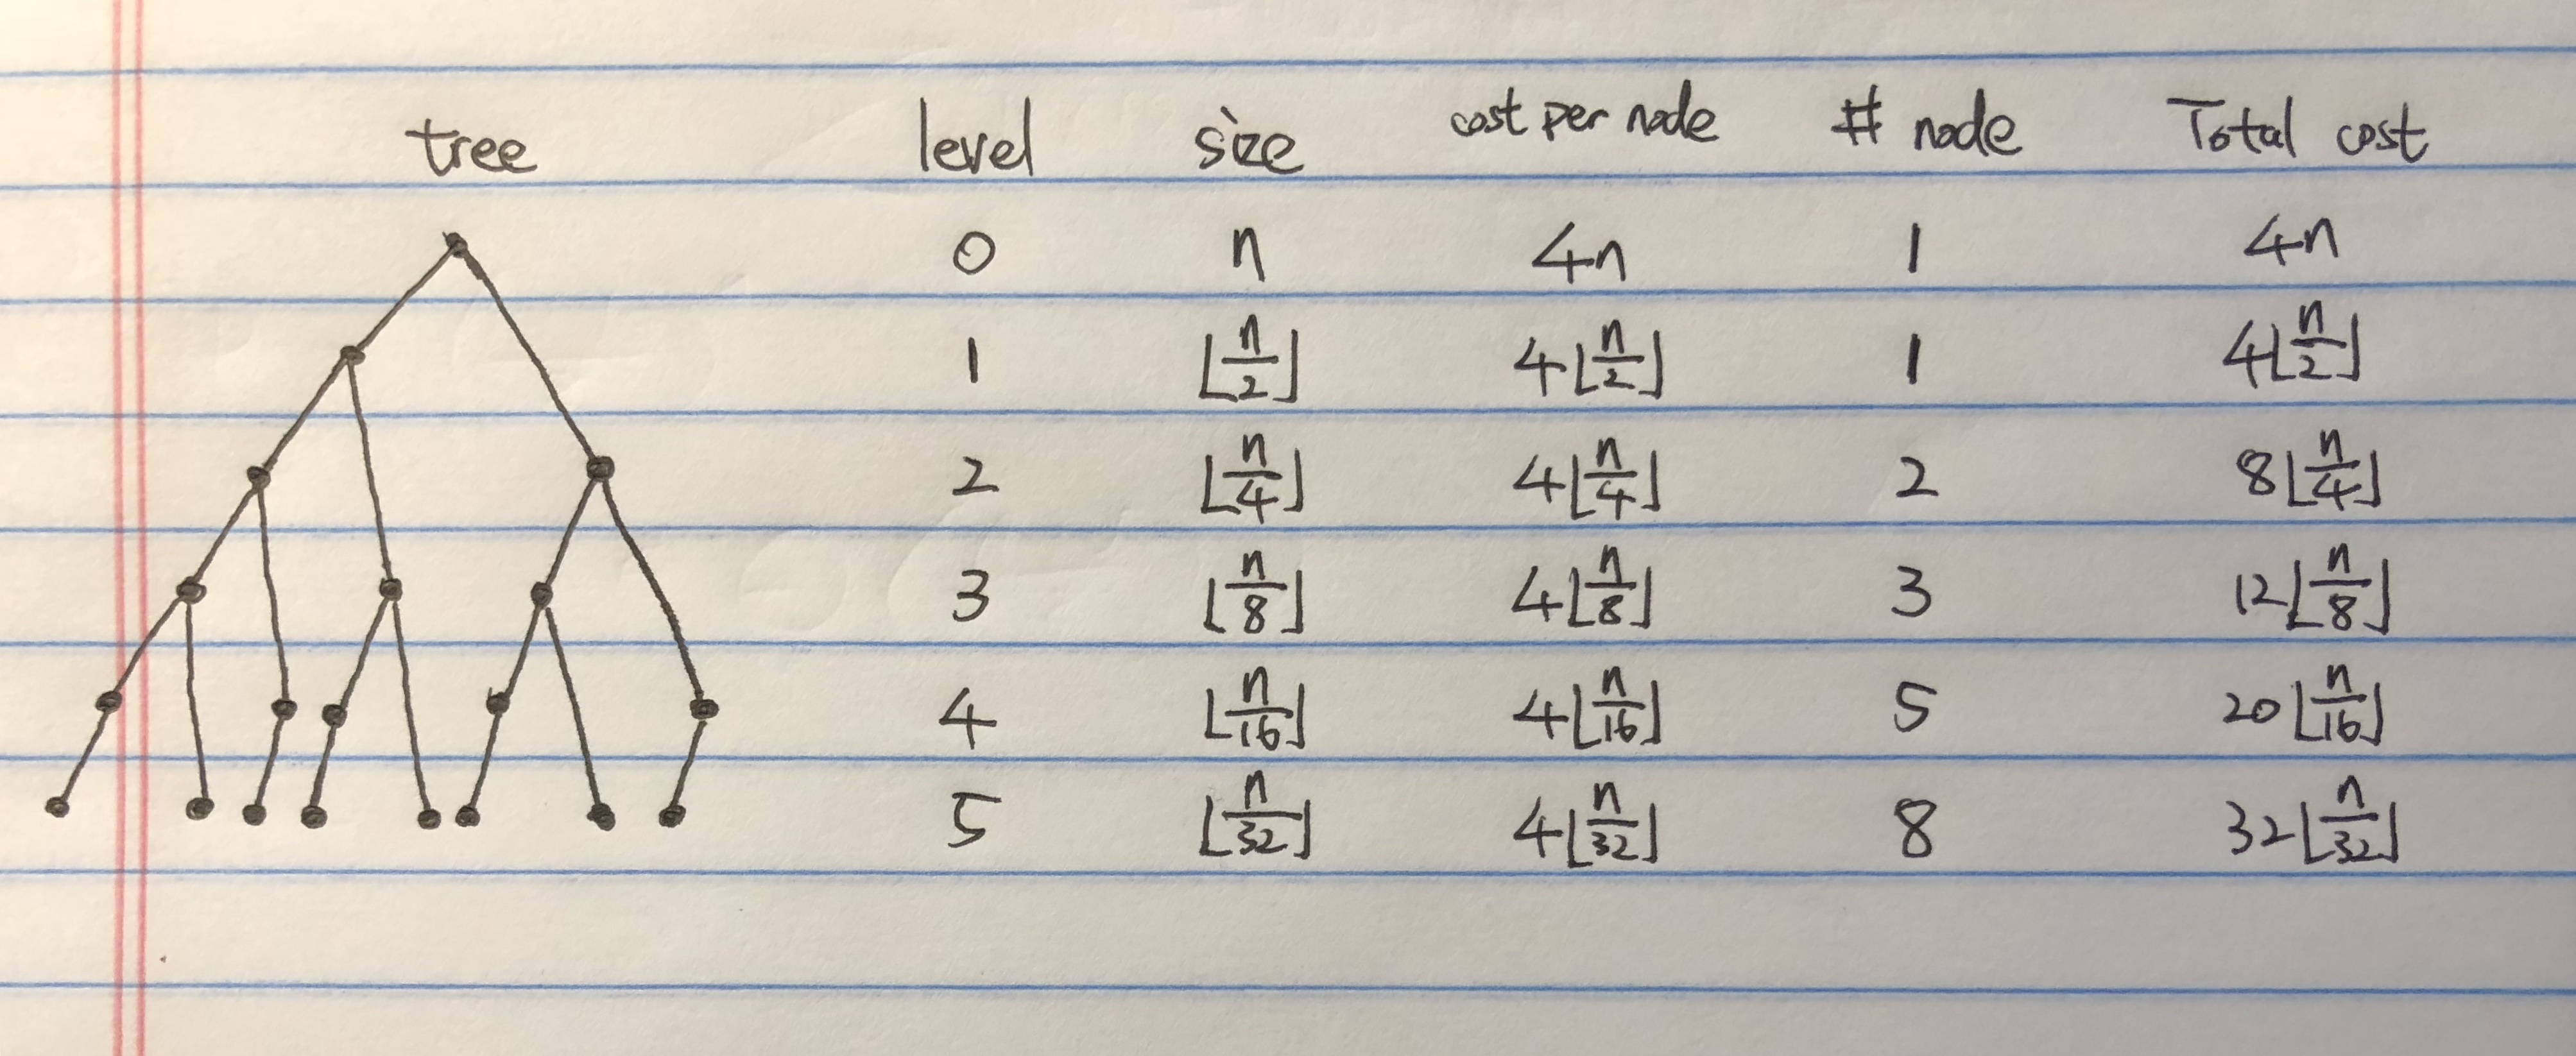
\includegraphics[width=0.9\textwidth]{tree.jpg}

\item [(1 points) 5.] Express the cost of all levels of the recursion tree as a sum over the cost of each level of the recursion tree.

\textbf{Cost function:} $F(k)c+\displaystyle\sum_{i=0}^{k-1}F(i)*\floor{\frac{4n}{2^i}}$, where $k$ is the level when size is $1$.


\item [(2 points) 6.] Give a function $g(n)$ and show it is an upper bound on the sum.

\textbf{Answer:}
\noindent
\begin{align*}
	cF(k)+\displaystyle\sum_{i=0}^{k-1}F(i)*\floor{\frac{4n}{2^i}} \leq cF(k)+4n\displaystyle\sum_{i=0}^{k-1}F(i)*\frac{1}{2^i}
\end{align*}

Since $\displaystyle\sum_{i=0}^{k-1}F(i)*\frac{1}{2^i} < 1 \Rightarrow 4n\displaystyle\sum_{i=0}^{k-1}F(i)*\frac{1}{2^i} < 4n$, and $c*F(k)$ is just a constant. It's suffice to say that $cF(k)+4n\displaystyle\sum_{i=0}^{k-1}F(i)*\frac{1}{2^i} \in O(n) = g(n)$.

\item [(3 points) 7.] State and prove by induction a theorem showing $T(n)\in\text{O}(g(n))$.
\begin{theorem}
	$T(n) \leq bn$.
\end{theorem}
\begin{proof}(By induction)
	For base case: $n=1,2,3$. We need $T(3)\leq b$ to prove all the base cases.
	
	Inductive hypothesis: Assume $T(K)\leq bk$ for $K<n$.
	
	Inductive step: when $n > 3$,
	\begin{align*}
		T(n) &= T\left(\left\lfloor\frac{n}{2}\right\rfloor\right)+T\left(\left\lfloor\frac{n}{4}\right\rfloor\right)+4n \\
		&\leq b\floor{\frac{n}{2}} + b\floor{\frac{n}{4}} + 4n \\
		&\leq b\frac{n}{2} + b\frac{n}{4} + 4n \\
		&= \frac{3}{4}bn + 4n \\
		&\leq bn \ \ \ \ \text{ only if } b \geq 16
	\end{align*}
	
	Let $b=max\{T(3), 16\}$, so $T(n) \leq bn$ for all $n\geq 1$ by induction.
\end{proof}

\item [(3 points) 8.] State and prove by induction (or other means) a theorem showing $T(n)\in\Omega(g(n))$.
\begin{theorem}
	$T(n) \geq an$.
\end{theorem}
\begin{proof}
	Since $T\left(\left\lfloor\frac{n}{2}\right\rfloor\right)+T\left(\left\lfloor\frac{n}{4}\right\rfloor\right)+4n > 4n$ for sure and $T(K)$ is always going to be positive for all $K>0$. Hence, $T(n)\in\Omega(n)$.
\end{proof}


\end{enumerate}

\noindent\textbf{Grading} You will be docked points for errors in your math, disorganization, unclarity, or incomplete proofs. 

\newpage

\subsection{Challenge}

In lecture we considered a proof that the expected worst case running time of the \textit{randomized quicksort algorithm} is $\Theta(n\log n)$.  The analysis used an integral approximation for a summation that we have not studied in this class.  There is a proof of this result that does not rely on this method.

The proof is based on the following observation.  With probability $\frac{1}{2}$ the pivot selected will be between $\frac{n}{4}$ and $\frac{3n}{4}$ (i.e. a good pivot).  Also with probability $\frac{1}{2}$ the pivot selected will be between $1$ and $\frac{n}{4}$ or between $\frac{3n}{4}$ and $n$ (i.e. a bad pivot). 

\begin{enumerate}
\item [(1 points) 1.] State a recurrence that expresses the worst case for bad pivots.

We actually talked about this in class. This is the worst case for quicksort.
\[
T(n) = \left\{
\begin{tabular}{cc}
c & \text{if} $n\leq1$ \\
$T(n-1)+dn$ & \text{if} $n>1$ \\
\end{tabular}\right.
\]
\item [(1 points) 2.] State a recurrence that expresses the worst case for good pivots.

Because With probability $\frac{1}{2}$ the pivot selected will be between $\frac{n}{4}$ and $\frac{3n}{4}$, it's using the median of medians algorithm and the list $M$ consists of $\frac{n}{4}$ medians of lists of size 4. By following the path we talked about in class, I got this recurrence:
\[
T(n) = \left\{
\begin{tabular}{cc}
c & \text{if} $n\leq1$ \\
$T(\floor{\frac{3n}{4}}) + T(\floor{\frac{n}{4}})+dn$ & \text{if} $n>1$ \\
\end{tabular}\right.
\]
\item [(2 points) 3.] State a recurrence that expresses the expected worst case by combining the first two recurrences.
\[
T(n) = \left\{
\begin{tabular}{cc}
c & \text{if} $n\leq1$ \\
$\frac{1}{2}(T(\floor{\frac{3n}{4}}) + T(\floor{\frac{n}{4}}) + T(n-1))+dn$ & \text{if} $n>1$ \\
\end{tabular}\right.
\]



\item [(6 points) 4.] Prove by induction that your recurrence is in $\text{O}(n\log n)$.
\end{enumerate}

\begin{proof}(By induction)
	For base case:$n=2,3,4$. We need $T(4) \leq 2b\log 2 \Rightarrow b\geq \frac{T(4)}{2}$.
	
	$n=1$ is not a option here because $\log 1 = 0$.
	
	Inductive Hypothesis: Assume $T(k) \leq bk\log k$ for $k<n$.
	
	Inductive step: when $n \geq 5$,
	\begin{align*}
		T(n) &= \frac{1}{2}(T(\floor{\frac{3n}{4}}) + T(\floor{\frac{n}{4}}) + T(n-1))+dn \\
		&\leq \frac{1}{2}((b\floor{\frac{3n}{4}}\log \floor{\frac{3n}{4}}) + b\floor{\frac{n}{4}}\log \floor{\frac{n}{4}} + b(n-1) \log (n-1)) + dn \\
		&\leq \frac{1}{2}((b\frac{3n}{4}\log \frac{3n}{4}) + b\frac{n}{4}\log \frac{n}{4} + b(n-1) \log (n-1)) + dn \\
		&= \dots
	\end{align*}
\end{proof}





\noindent\textbf{Grading} Correctness and precision are of utmost importance.  Use formal proof structure for the big-Theta bounds.  You will be docked points for errors in your math, disorganization, unclarity, or incomplete proofs.    
%%% End document

\end{document}